\documentclass[../main.tex]{subfiles}

\begin{document}

\section{AutoLibra as A Ladder \protect

\includegraphics[height=1em]{figs/ladder.png}
: Agent Improvement with AutoLibra}
\label{sec:ladder}

% \begin{table}[!h]
% 	\centering
% 	\begin{tabular}{rcccc}
% 		\toprule        & \multicolumn{2}{c}{Baba-Is-AI (\ref{sec:Baba-Is-AI})} & \multicolumn{2}{c}{WebVoyager (\ref{sec:webvoyager})} \\
% 		                & Avg. Metrics                                          & Success Rate                                         & Avg. Metrics & Success Rate \\
% 		\midrule Iter 0 & 15.8\                                                 & 33.3                                                 & 45.9         & 34.8         \\
% 		Iter 1          & 28.2                                                  & 40.0                                                 & 53.8         & 35.5         \\
% 		Iter 2          & 40.7                                                  & 44.4                                                 & 61.3         & 38.1         \\
% 		Iter 3          & 56.7                                                  & 52.7                                                 & 69.9         & 39.7         \\
% 		\bottomrule
% 	\end{tabular}
% 	\caption{Using AutoLibra-induced metrics as optimization targets for prompt
% 	engineering and finetuning leads to improvements in the average metric
% 	positive rates (Avg. Metrics) and task success rate (Success Rate) defined by the
% 	two environments respectively.}
% 	\label{tab:baba_wv_scores}
% \end{table}

% \begin{figure}[!t]
% 	\centering
% 	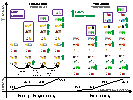
\includegraphics[width=0.8\textwidth]{figs/autolibra-teaser.pdf}
% 	\caption{AutoLibra iteratively discovers new optimization targets throughout
% 	the agent optimization process. Each emoji pair represents an induced metric;
% 	the arrows and text between iterations represents the changes made to prompts
% 	informed by metrics. Purple boxes indicate the newly emerging metrics, and
% 	green arrows indicate significant improvements over the previous iteration. The
% 	metric names can be found in Tab. \ref{tab:baba_is_ai_metrics} and App. Tab.
% 	\ref{tab:app_nnetnav_metrics}. }
% 	\label{fig:autolibra-training}
% 	% 	\vspace{-20pt}
% \end{figure}

% \subsection{Can AutoLibra induce good optimization targets for prompt
% engineering?}
% \label{sec:Baba-Is-AI}

% To answer this question, we use \textbf{Baba-Is-AI} \citep{cloos2024babaaibreakrules, paglieri2024balrog}
% as a case study, since it is not yet saturated by state-of-the-art LLM agents. This
% game requires metacognitive skills, such as breaking and building new rules and
% planning ordered subtasks; a full list of game rules is listed in App.
% \ref{appendix:baba_is_ai_rules}. We use the top model on the leaderboard\footnote{\url{https://balrogai.com}}
% (which when we started the experiments, was GPT-4o) \citep{openai2024gpt4ocard}
% for the agent policy, while we observe similar improvements in Claude-3.5-Sonnet\footnote{\url{https://www.anthropic.com/news/claude-3-5-sonnet}}
% as well.

% % \begin{figure}[ht]
% %     \centering
% %     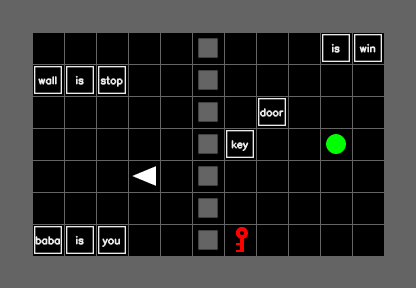
\includegraphics[scale=0.5]{figs/babaisai_env.png}
% %     \caption{Example of the Baba-Is-AI environment. In this task (two\_room-break\_stop-make\_win-distr\_obj-irrelevant\_rule), the agent has to break the "wall is stop" rule and push the "key" rule block next to "is win" to assemble the win rule, then touch the key to win. Pushing the "door" rule block would be a mistake, as no door object is present.}
% %     \label{fig:babaisai_env}
% % \end{figure}

% % \subsection{AutoLibra for Baba-Is-AI improvement}

% To avoid overfitting to the tasks used in optimization, we fine-tune on 6 of 40 tasks
% in Baba-Is-AI \citep{paglieri2024balrog}, but report performance on all 40 tasks.
% In one \textit{Iteration}, the human prompt engineers (two of the authors)
% generate 18 agent trajectories (3 trajectories / task), use AutoLibra to induce metrics,
% then optimize the prompt to achieve higher performance on the induced metrics
% without considering the task success rate, and start a new iteration when one or
% more metrics improved significantly (over 30\%). The procedure and experiment setup
% are detailed in App. Alg. \ref{appendix:algo1} and App.
% \ref{appendix:autolibra_setup}.
% \vspace{-0.4cm}

% \paragraph{Results}
% As shown in Fig. \ref{fig:autolibra-training} and Tab. \ref{tab:baba_wv_scores},
% the performance on Babaisai task increased from 25\% to 55\% between \textit{Iteration
% 0} and \textit{Iteration 3}, with each iteration resulting in greater performance
% than the previous; this is replicated across the held-out tasks alone, (complete
% task results tabulated in App. \ref{appendix:heldout}). This represents a substantial
% increase compared to the highest base model performance of 33\% on Baba-Is-AI
% \citep{paglieri2024balrog}. With only 6 tasks used in inducing the metrics, the improvement
% on all 40 tasks showing the metrics induced by AutoLibra are generalizable to unseen
% tasks. Among induced metrics (App. Tab. \ref{tab:baba_is_ai_metrics}), agent performance
% increases correspondingly to prompt changes targeting those metrics, an example
% being \texttt{Win Condition Recognition}
% 
\includegraphics[height=1em]{figs/emojis/emoji_1.png}
% , which increases from 28\% to 50\% from \textit{Iterations 0-1} after few-shot
% prompting (prompt in App. \ref{box:baba_is_you_iter_1}) is introduced to teach the
% identification of a win condition rule. The complete list of observations and
% reasoning for prompt engineering is in the App. \ref{appendix:baba_is_ai_obs}.
% With AutoLibra, prompt engineers could receive feedback on whether their prompt changes
% lead to desired behavior changes in agents.

% % \begin{wraptable}
% % 	[19]{r}{0.60\textwidth} % 'r' for right, adjust the width as needed
% % 	\centering
% % 	\small
% % 	\vspace{-10pt}
% % 	\begin{tabular}{ccl}
% % 		\toprule \multicolumn{1}{c}{Emoji}                                                & \multicolumn{1}{c}{It.} & \multicolumn{1}{l}{Metric}             \\
% % 		\midrule \rowcolor{gray!10} 
\includegraphics[scale=0.07]{figs/emojis/emoji_1.png} & 0                       & Win Condition Recognition              \\
% % 		\midrule \rowcolor{gray!10} 
\includegraphics[scale=0.07]{figs/emojis/emoji_2.png} & 0                       & Rule Modification                      \\
% % 		\midrule \rowcolor{gray!10} 
\includegraphics[scale=0.07]{figs/emojis/emoji_3.png} & 0                       & Direct Navigation Efficiency           \\
% % 		\midrule \rowcolor{gray!10} 
\includegraphics[scale=0.07]{figs/emojis/emoji_4.png} & 0                       & Context-Sensitive Decision Making      \\
% % 		\midrule \rowcolor{gray!30} 
\includegraphics[scale=0.07]{figs/emojis/emoji_5.png} & 1                       & Win Rule Construction                  \\
% % 		\midrule \rowcolor{gray!30} 
\includegraphics[scale=0.07]{figs/emojis/emoji_6.png} & 1                       & Selective Interaction w/ Relevant Obj. \\
% % 		\midrule \rowcolor{gray!30} 
\includegraphics[scale=0.07]{figs/emojis/emoji_7.png} & 1                       & Rule Manipulation and Execution        \\
% % 		\midrule \rowcolor{gray!60} 
\includegraphics[scale=0.07]{figs/emojis/emoji_8.png} & 2                       & Subtask Coordination                   \\
% % 		\midrule \rowcolor{gray!90} 
\includegraphics[scale=0.07]{figs/emojis/emoji_9.png} & 3                       & Immovable Interaction                  \\
% % 		\bottomrule
% % 	\end{tabular}
% % 	\caption{Metrics and Turn of Induction
% % 	\newline
% % 	for Baba-Is-AI}
% % 	\label{tab:baba_is_ai_metrics}
% % \end{wraptable}

% % Similarly to results observed in Section 3, induced metrics are observed to capture the behavior of the agent increasingly well with additional iterations, with coverage increasing from 65\% at \textit{Iteration 0} to 92\% at \textit{Iteration}, while mean redundancy remains 56\% across all iterations. The trajectory performance also improved significantly, with the average number of steps per task (capped at 100) decreasing from 79 to 51, indicating that the agent's reasoning performance and efficiency improved as a result of the code changes made in each iteration.

% Qualitative observation of agent trajectories reveals behaviors commensurate with
% induced metric scores; the agent random-walks in \textit{Iteration 0}, navigates
% towards specific objectives but gets stuck or trapped in a loop on long-horizon
% tasks in \textit{Iteration 1} and \textit{Iteration 2}, and fully understands basic
% subtasks (atomic goals on the critical path to environment completion) and the correct
% order of subtasks to successfully complete an environment in \textit{Iteration 3}.
% A per-metric score breakdown is listed in Appendix \ref{appendix:babaisai}, and
% a full per-iteration documentation of code changes and results is presented in
% Appendix \ref{appendix:baba_is_ai_obs}.

% % \subsubsection{Held-Out Task Performance}

% % \paragraph{Ablation Study}

% % To evaluate the generalization of the improvements realized by AutoLibra, we conducted an ablation study where the performance of the agent improved by AutoLibra was evaluated on unseen Baba Is You levels, arbitrary LLMs, and entirely new environments.

% \textbf{Generalization to other models} When replacing GPT-4o with Claude-3.5 as
% the LLM used in the agent (Appendix \ref{appendix:heldout}), performance was found
% to be similar across all iterations, with held-out task performance increasing
% by 20\% to 55\% between \textit{Iteration 0} and \textit{Iteration 3} and
% qualitatively similar trajectory performance and agent behaviors observed
% between the two LLMs. This demonstrates that the improvements realized by AutoLibra
% are generalizable to other LLMs, and that the induced metrics are robust to
% changes in the underlying LLM.

% \textbf{Generalization to other tasks} To evaluate whether this pipeline can be generalized
% to other domains, we conduct the same pipeline to MiniHack \citep{samvelyan2021minihackplanetsandboxopenended},
% an environment whose tasks and action space are more complex than Baba-Is-AI. Similarly
% to Baba-Is-AI, in three iterations, the task completion rate was observed to increase
% to 25\%, an improvement of 15\% versus the baseline of 10\%, validating
% AutoLibra's general utility in improving agent performance; full results are available
% in the Appendices \ref{appendix:minihack_rules}-\ref{appendix:minihack_obs}.
% %\diyi{use a paragraph title to illustrate that this is about generalization? i also didn't quite follow why minihack is only summarized using these two sentences. if you want to emphasize it, explain it clearly; otherwise, no need to mention it? }

% \subsection{Can AutoLibra induce good optimization targets for agent fine-tuning?}

\begin{figure}[!b]
	\centering
	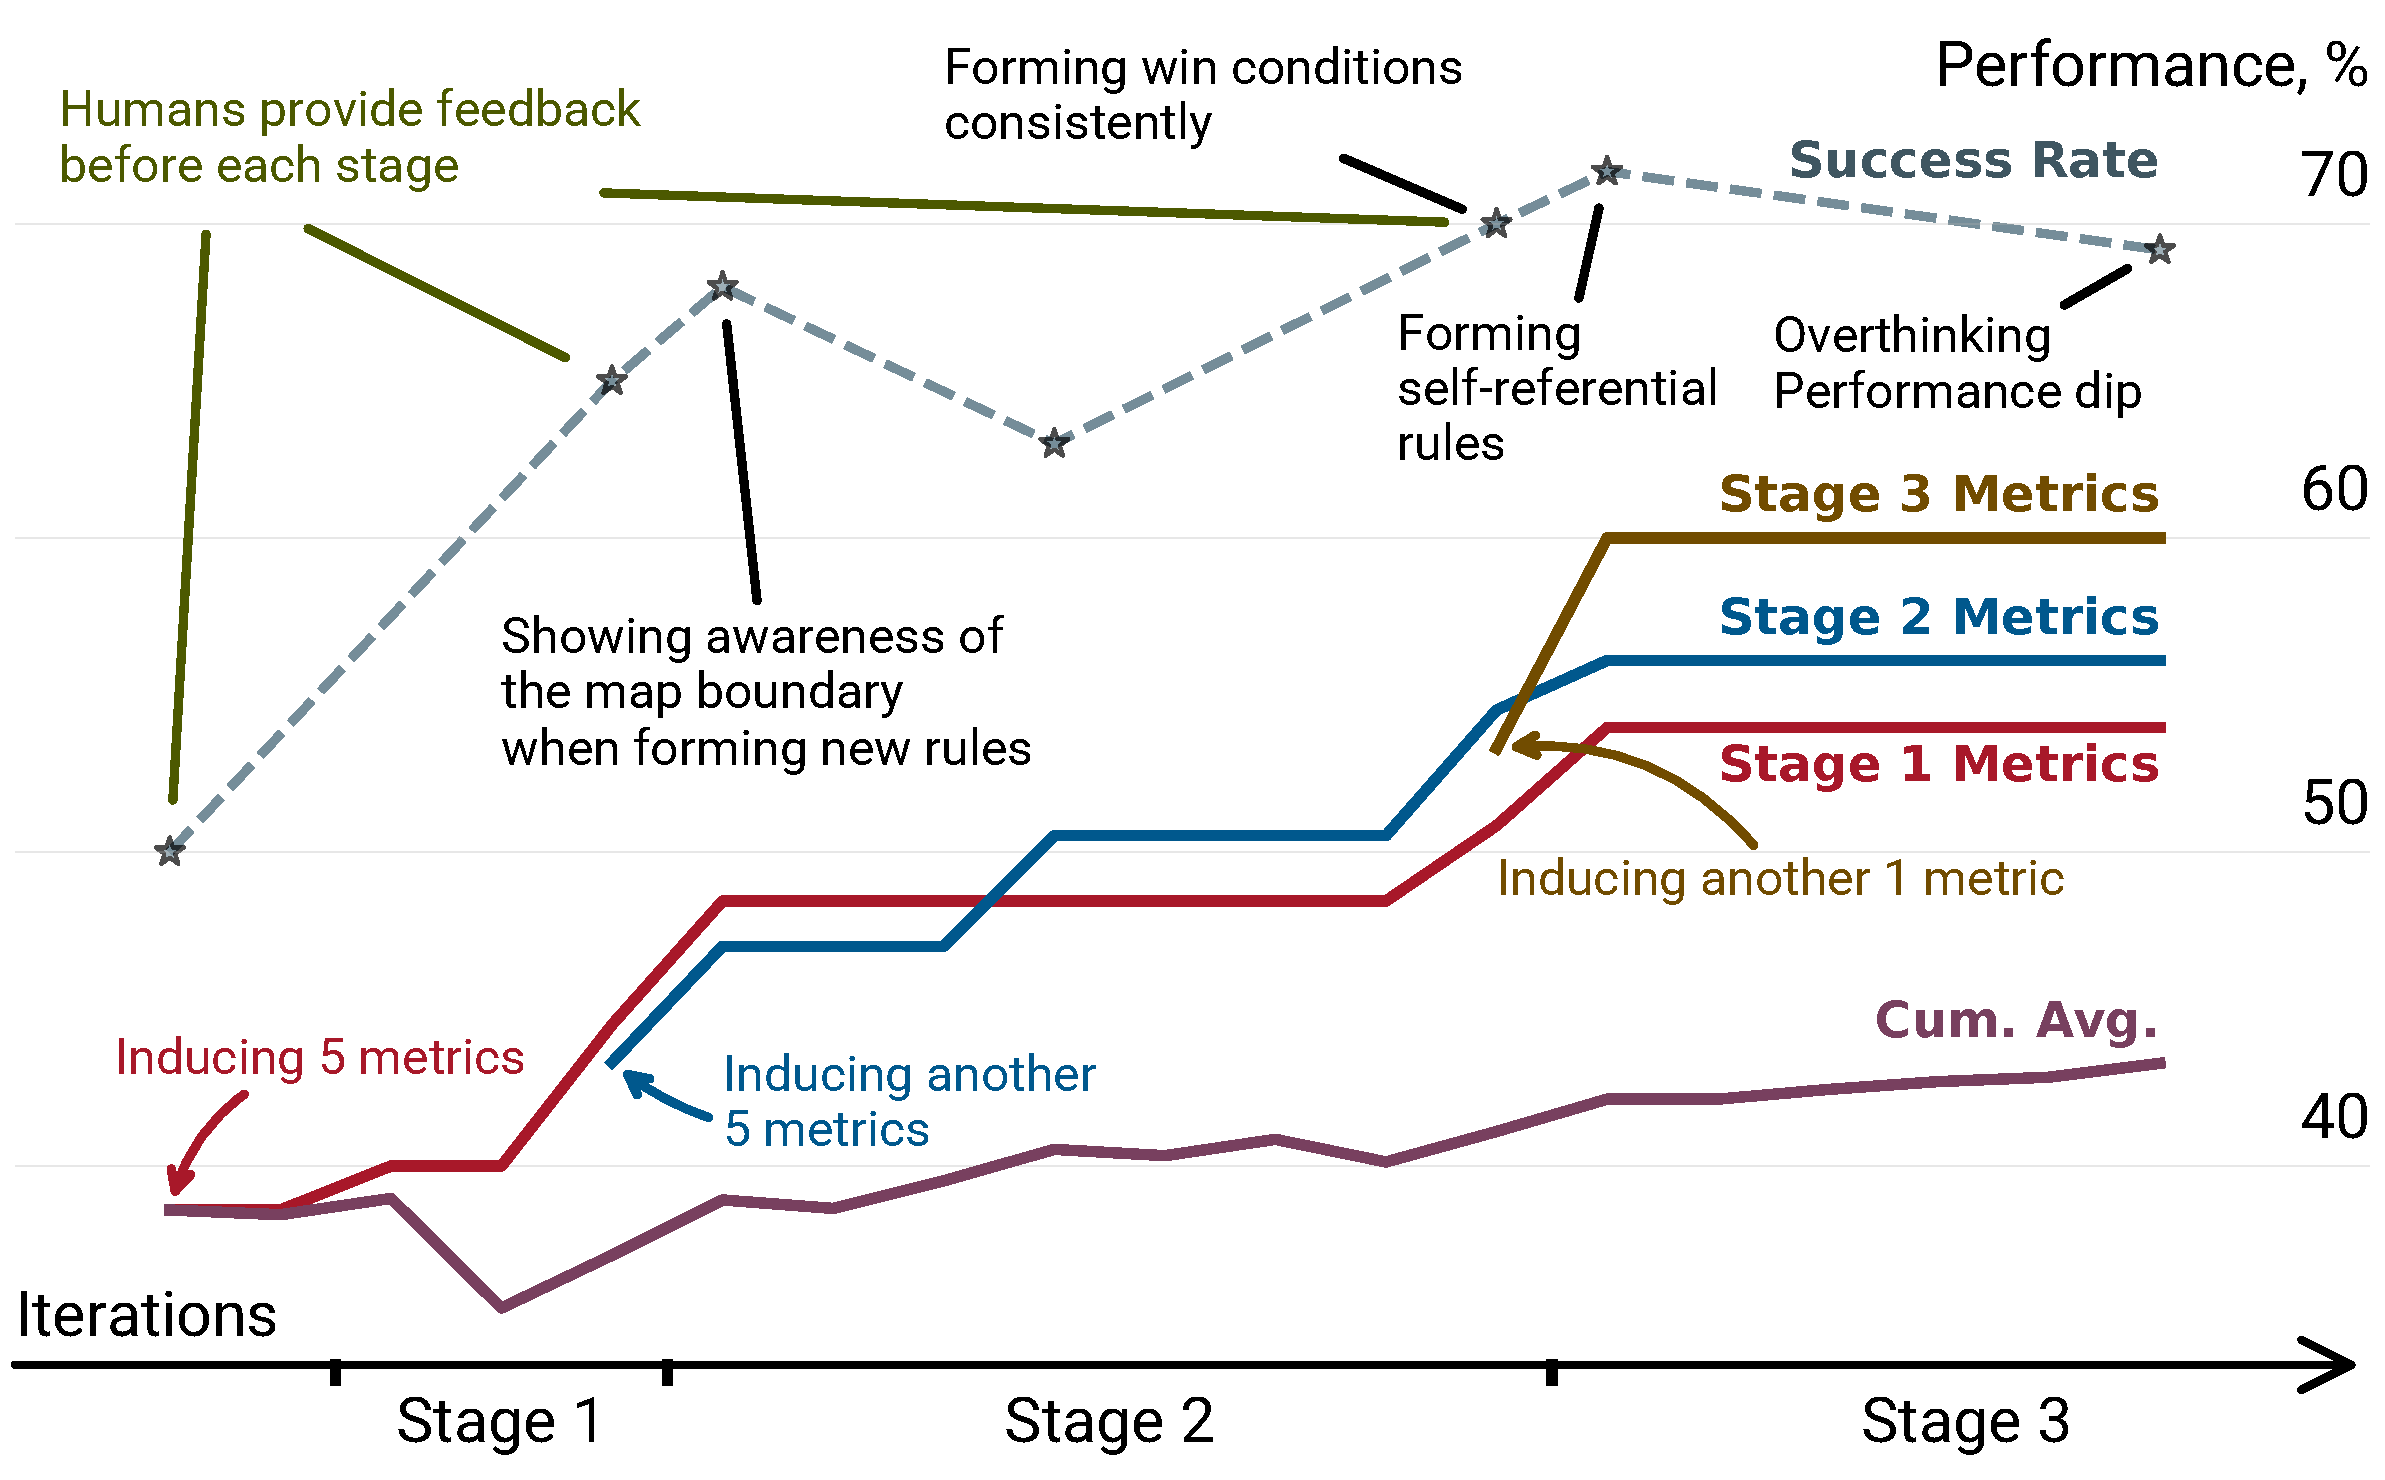
\includegraphics[width=0.8\textwidth]{figs/running_maximum_plot.pdf}
	\caption{AutoLibra iteratively induce metrics and improves the agent prompts
	through optimizing for the induced metrics. Although not optimized for, the
	success rate of the agent continuously improve until Stage 3, when the agent begins
	to overthink.}
	\label{fig:autolibra_self_improving}
\end{figure}

As AutoLibra can automatically induce metrics from human feedback, a natural
question to ask is whether it can enable self-regulated improvement in agents
through iterative feedback. This can be achieved through optimizing the agent prompts
towards higher scores on the metrics extracted by AutoLibra. To answer this
question, we use a challenging 2D game Baba-Is-AI \citep{cloos2024babaaibreakrules, paglieri2024balrog}
as a benchmark. Inspired by \href{https://hempuli.com/baba/}{Baba-Is-You}, this
game requires not only following rules to achieve goals, but also manipulating the
rules, even self-referential ones. For example, in the game illustrated in App. Fig.
\ref{fig:baba-is-ai}, the agent needs to change self-referential rules from \textsl{baba
is you}, to \textsl{door is you} to control the green door on the other side of
the wall, form a new win rule \textsl{ball is win}, and navigate to the red ball
to achieve the win condition. To achieve a high score on this dataset, the agent
needs not only planning, but also metacognitive skills, which is very challenging
for LLM agents with frontier models as shown in the Balrog benchmark \citep{paglieri2024balrog}.
In this experiment, we use Gemini-2.5-Flash \citep{geminiteam2025geminifamilyhighlycapable}
for the agent, AutoLibra, and agent prompt optimization, throughout the
experiment, which will be referred as the LLM in this section. Gemini-2.5-Flash
is ranked as the 3rd place, with a success rate of $50.8\%\pm 4.6\%$ on the Balrog
leaderboard for Baba-is-AI at the time of submission, and the state-of-the-art
result is $56.7\%\pm4.5\%$.

\begin{figure}[!t]
\centering
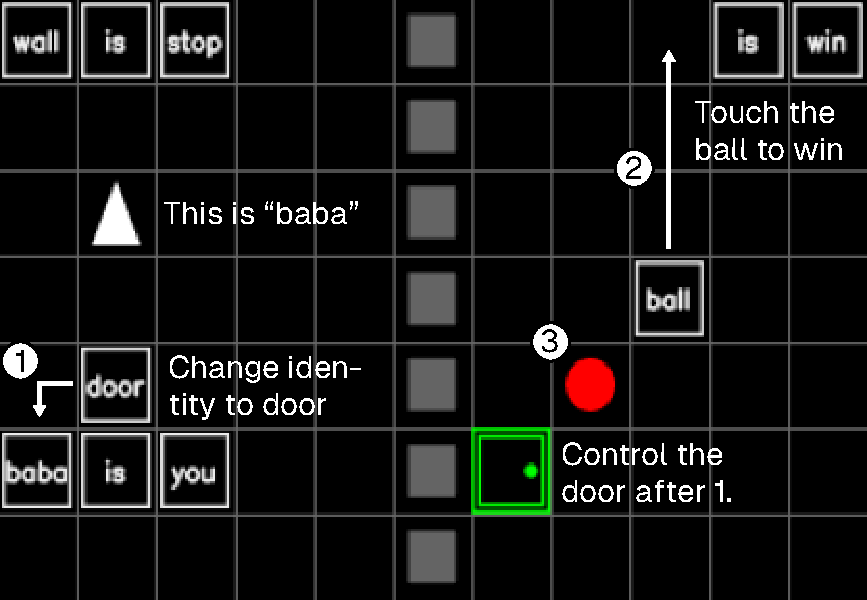
\includegraphics[width=0.5\textwidth]{figs/babaisai-self-referential.pdf}
\caption{Example of Baba-Is-AI game.}
\label{fig:baba-is-ai}
\end{figure}


Fig. \ref{fig:autolibra_self_improving} illustrated our procedure, and
summarized the results. We employ an iterative process by improving the agents in
3 stages through providing human feedback on 6 out of 40 tasks in the Baba-Is-AI.
Before each stage we show human annotators 3 trajectories for the 6 tasks, gather
the feedback, and apply AutoLibra iterative metric induction process (\S\ref{sec:iterative-induction}).
This results in 5 metrics for Stage 1 and 2, and another 1 metric for Stage 3. Within
each stage, we iteratively feed 1 LLM agent trajectory on each of these 6 tasks,
together with evaluation results based on these AutoLibra-induced metrics to the
LLM to improve the prompt of the LLM agent. This process results in continuous
improvement not only on the running maximum metric scores, the cumulative average
metrics, but also game success rate. Fig. \ref{fig:autolibra_self_improving}
shows these statistics on the whole 40 tasks, although we only use 6 out of the 40
tasks in the whole optimization process. Upon examining the agent trajectories, we
find the skills learned in the process. In the first stage, the agent learns to find
rules to form based on the map boundary, which could be a result of an induced
metric \texttt{map-n-constraint-recognition}. Similarly, more advanced skills are
learned in Stage 2 and 3, including forming win conditions and self-referential
rules, probably as a result of metric \texttt{rule-manipulation-proficiency}.

Our results show that the metrics induced by AutoLibra form effective objectives
for improving the agents through prompt optimization. It should note that AutoLibra
is a metric induction method, which is orthogonal to learning algorithms, including
prompt optimization, fine-tuning or reinforcement learning. We show that this process
improves agent success rate by 20\% without optimizing for success rate, and in the
future, researchers can study the effect of employing other learning algorithm.

\end{document}